\section{Conceptual Overview}
In this section we present a conceptual overview of the subjects of this
study--Workflows and Scientific Workflow Environments.

\subsection{Distinction with Traditional Programming Environments}
SWEs differ in many respects among themselves as well as with respect to traditional
programming environments. Consequently, a choice of the suitable SWE must be
made. The following list identifies the major differences
between traditional and the SWE programming paradigm:

\begin{enumerate}
%
\item \textbf{Scalability and Optimization.} SWEs are more likely to involve
extensive usage of distributed resources than conventional programs. Owing
to the large-scale experiments, for which scientific users turn to automation,
their demands for computational power often exceeds that of a single personal
computer. These properties make them ideal candidates for a large-scale
distributed computing environment. The case for suitability of SWEs on
large-scale distributed infrastructures has been well-argued upon
in~\cite{jha-katz-etal:2009}. In such a scenario, taking explicit steps to
ensure scalable and optimized performance is vital. Additionally, most SWEs are
capable of executing workflows at small scale with minimal tuning. This
multi-scalability enables quick and easy conceptualization and prototyping of
new workflows.
%

\item \textbf{Performance and Throughput.} While programming platforms for
large-scale computing exist mostly as HPC (high-performance computing)
domain systems such as MPI, OpenMP, CUDA, etc. the dominant area for SWEs in
this field is HTC (high-throughput computing). The main underlying difference
here is the granularity of a task. HPC platforms run tasks at a finer
granularity such as a CUDA thread or an MPI process where as SWEs run a task at
a coarser granularity such as an invocation of a legacy executable.

\item \textbf{Data Management.} The scale of data transfer is much higher in
SWEs from one execution site to others as well as among storage resources while
it is lower (ranging from variables to small data structures) in programs.
Owing to such scales, applications often need access to special data movement
and access and movement protocols such as GridFTP, Amazon S3, NAS, etc. SWEs are often
shipped with capabilities to handle such protocols.
%

\item \textbf{Interface to Distributed Computing Infrastructures (DCIs).}
Supporting an interface to a distributed system is a complex task from the
point of view of an SWE. The distributed nature of resource utilization and
asynchronous execution of workflow requires a set of interdependent parameters
to be configured correctly. Modern computing infrastructures such as Clouds,
GPUs and supercomputers with hybrid nodes (CPU + GPGPU) pose new challenges of
interface development.  As SWEs involve running many tasks over an
infrastructure it becomes crucial to interface with these systems such that the
tasks are scheduled in an optimal manner. Many SWEs implement
\emph{pilot-jobs}~\cite{montagnat-glatard-etal:2010,ucc2011} in order to
reserve resources via pseudo-tasks that act as placeholders for real tasks.
Additionally, decision to manage working data storage on disc, memory and cache
are some of the distinctions between a traditional programming and workflow
platforms in the context of distributed and scalable computation.

\item \textbf{Expressiveness.} Programming languages are inherently control
flow oriented where data flow is a secondary aspect. Often, the
programmer must explicitly make sure that correct inputs are available
to instructions and are in the right format. A program proceeds as the
execution of its statements from beginning to end and completes its
execution in a predefined sequence. However, in SWEs, the flow is often
determined by the data availability for execution. This model of computation is
known as dataflow computing. A workflow thus does not follow a fixed order of
execution. Different execution sequences are possible which are dominated by
dataflow. The unit of work in SWEs is at a higher level of granularity. A unit
of execution is coarse-grained, and often termed as ``processor'', ``task'',
``service'' or ``actor'' in the SWE community. This notion of high-level
granularity drives the depth to which a workflow can be expressed in a given
language form. In the rest of the paper, we refer to this unit of execution of a
workflow system as \emph{processor}. On the other hand, a unit of execution in
most programming languages is a much simpler and finer executable statement
that accomplishes a small task. This presents a whole new set of
requirements for expressing the processors and how they should interact with
computational resources and operate upon data.

%
\item \textbf{Usability.} SWEs predominantly serve as a tool for the domain
experts to utilize the computational power. This makes it essential for
them to have a friendly, and intuitive user-interface for novice and
non-expert users. For this reason, SWE user interfaces are dominated by the
visual paradigm of programming. On the other hand, as the sophistication of
expression and user expertise increases, the visual environment temds to get
limited in capabilities it can offer. Thus, most SWEs have a text-based
composition environment albeit with visually assisting programming environments
such as IDEs. However, these textual environments are seldom to the extent that
a non-expert user can graphically compose programs. While a graphical interface
enhances usability, a text-based workflow environment can arguably give better
control to an experienced user. Consequently, many workflow systems offer a
dual interface of graphical and text medium to compose workflows.
    
\end{enumerate}

We concede that the above is not an exhaustive list of differences in features.
However, it is reasonably inclusive and we believe it covers the breadth of the
aspects we discuss in the current work. We do not include other interesting SWE
features such as application predictability in this analysis as they are out of
scope of the objectives of the current paper.

\subsection{Workflow}
Figure~\ref{fig:wf} shows a typical workflow in the form of a Directed Acyclic
Graph (DAG). Execution typically begins with the input data being provided to
the first task and ends at the results being delivered at the end of the last
task. Tasks are represented by boxes and data/control flow between the task is
represented as arrows. Note that in cases where tasks are connected with pure
control flow, it can be simulated by passing token data between tasks.

For the purpose of this text, we define a workflow as a specification of
computation with at least two discrete tasks either forming distinct
computational stages or running for two or more distinct datasets as
parameters. Consequently, a one-off task or running a task for a single copy of
data is \emph{not} a workflow.

For the rest of this paper, we will use the above definition of a workflow.
%

\begin{figure}[htb]
\begin{center}
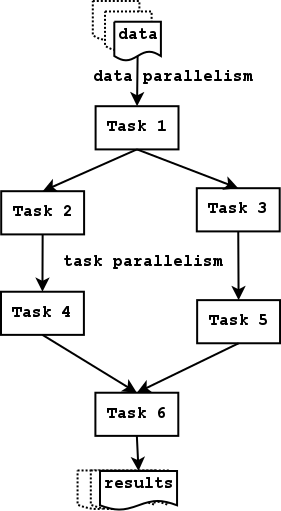
\includegraphics[width=4cm]{figures/workflow}
\caption{A typical workflow depicted as a Directed Acyclic Graph (DAG) of tasks coordinated by data or control flow and illustrating data and task parallelism}
\label{fig:wf}
\end{center}
\end{figure}
%

\subsection{Architecture}
Figure~\ref{fig:wfms} shows a high-level architecture of a generic SWE. It shows key
components and their interaction in an SWE. These components are the focus of
interest for the present work. A \textit{user interface} interacts with the
\textit{workflow engine} using commands and messages on the inside while with
user on the outside. The \textit{workflow language} becomes an intermediate
representation for communication between user interface and the
\textit{workflow engine}. The workflow engine acts as a compiler/interpreter
and a high-level scheduler for the processors and interfaces with the
underlying \textit{distributed resources}. It resolves data dependencies and
optimizes the flow at runtime and monitors the workflow progress and collects
the intermediate and final results.

%
\begin{figure}[htb]
\begin{center}
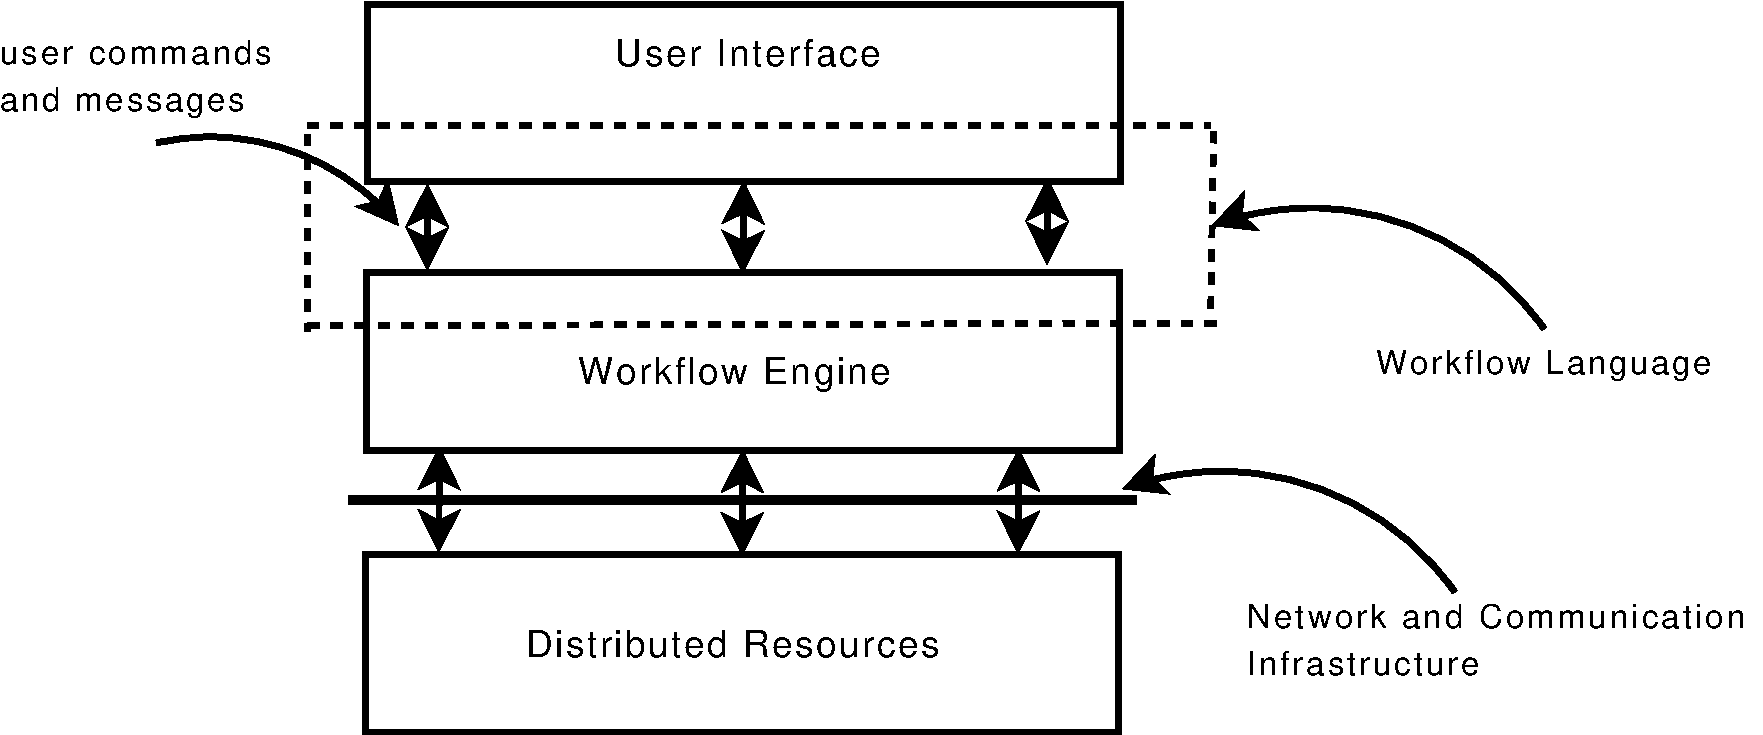
\includegraphics[width=\linewidth]{figures/workflow_interfaces_and_language}
\caption{A generic SWE scheme showing the relationship and interaction among important components}
\label{fig:wfms}
\end{center}
\end{figure}
%
SWEs are used as tools to benefit from the underlying large-scale computing
infrastructure such as clusters, supercomputers, clouds, and grids. Such
environments are in use today for production level work in different scientific
domains worldwide. They do the basic task of linking inter-related processors
of a multi-staged scientific computation. However, they differ in the features
they provide based upon the scientific domain or user community they offer
service for, and the computational model they follow. Often, one of the main
reasons for such difference is the specialized components and requirements for
a particular domain. Owing to this fact, a given workflow system dominates a
particular area of science (eg. astronomy, biology, etc.). Nonetheless, there
exist a plethora of SWEs suitable for general purpose workflow style
computations.

DAGs are by far, the most popular abstraction of the way workflows are
perceived and visualized. The MA DAG~\cite{caron-desprez:2005}, engine is one
example of a DAG generator engine. MA DAG has evolved from a regular DAG
generator to a more abstract DAG generator laced with control structures. MA
DAG benefits from the workflow scheduling mechanisms included in the
middleware. Due to the impossibility to produce complete DAGs owing to the
presence of control structures such as conditionals and loops, MA DAG generate
partial DAGs greedily: a sub-DAG, as complete as possible, is produced as soon
as possible. Despite the presence of many different approaches to workflow
systems, new requirements continue to pose workflow challenges. Some of the
current challenges facing SWEs are:

\begin{enumerate}
\item \textbf{Multisite execution.} Interfacing to existing computation and
storate infrastructure is not trivial, not to mention the new and
unforeseen access and compute modes. SWEs are yet to formulate a
generalized interface towards the major platforms such that they will
run on them out of the box.

\item \textbf{Manysite execution.} Even if a SWE has interfaces built for
more than one infrastructure, it is hard to optimally schedule large
workflows to many remote sites simultaneously. The problem of limited
control over remote sites and distributing interdependent data and
tasks makes it non-trivial to efficiently load-balance work among them.

\item \textbf{Expressivity.} Workflow languages have evolved over the years
with reasonable expressivity being supported. However, they are often
compared with those of the traditional programming languages. As of
current state of the art, the workflow languages expressivity still
have to catch up to the richness of programming languages across
different generations such as C and python.  The community is yet to
realize a truly generic workflow language that can express a wide
variety of flow patterns encountered in scientific domains.

\item \textbf{Interoperability.} Interoperable workflows will benefit to a
broad audience of users. Many efforts at this are made in the recent
past, such as by the consurtium projects and by individual players.
However, a truly interoperable set of standards for workflows are yet
to emerge.
\end{enumerate}
